\section{Moravec}\label{sec:moravec}
Moravecs hjørnedetektor\cite{moravec}, er en af de tidligste feature detektorer og i denne metode defineres et hjørne, som et dataindsamlingsvindue i et billede $I$, der er forskelligt fra dets lokalområde.
\\
Moravec anvender denne definition til at opnå en matematisk formulering af hjørner ved for hvert punkt i et billede, at udregne en auto-korrelationen mellem to kvadratiske dataindsamlingsvinduer. Et hjørne lokaliseres for et område og dets indsamlingsvindue, ved at forskyde vinduet én pixel i alle principielle retninger (horisontalt, vertikalt og diagonalt) og udregne intensitetsvariationen (auto-korrelationen) af alle de forskudte vinduer.  SSD(Summed Square Difference) benyttes til at finde forskellen på de kvadrede værdier i vinduerne:
\begin{equation}
\bold{E}(u,v)= \sum_{\forall \text{x,y i dataindsamlingsvinduet}} w(x,y)[I(x+u,y+v) - I(x,y)]^2
\label{moravec}     
\end{equation}
hvor $(u,v)\in \lbrace -1,0,1 \rbrace$ er forskydningen af vinduet, der summere over alle pixels i dataindsamlingsvinduet $w$. $w$ er her en matrix, med samme størrelse som $I$ og indeholder 1 indenfor hvis en pixelkoordinat $(x,y)$ ligger indenfor dataindsamlingsvinduet, og 0 ellers.
\\
Figur \ref{fig:moravec} illustrerer et dataindsamlingsvindue i rødt, her af størrelse af (3x3). Det blå vindue viser et diagonalt skift. Det ses, at det røde vindue til højre, ligger et på et ideelt hjørne. 
\begin{figure}[H]
    \centering
    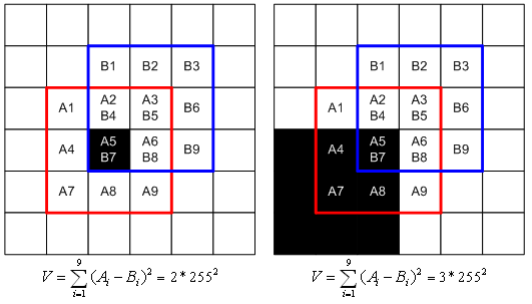
\includegraphics[width=0.55\textwidth]{fig/25.png}
     \vspace{-1em}
    \begin{center}    
       \caption{\textcolor{gray}{\footnotesize \textit{ SSD udregninger for intensitetsvariationer imellem forskudte vindue. }}}
    \label{fig:moravec}
     \end{center}
     \vspace{-2.5em}
  \end{figure} \noindent   
$E(u,v)$ beregnes otte gange for hver pixel. Den mindste forskel af de otte variationer, definere punktets hjørnestyrke $C(x,y)$.
$$
C(x,y)=min(E(u,v)) \text{$ $for alle permutationer af $u,v \in [0,1]$, pånær (u,v) = (0,0)}
$$
$C$ vil have et højt respons i de områder, hvor pixelintensiteter i originalvinduet ($w(x,y) = 1$), adskiller sig fra intensiteter, i de forskudte vinduer - jo større pixelintensitens forskellen er, jo højere $C$ værdi.
Det kan udledes her, at en horizontal, eller vertikal kant ikke vil blive karakteriseret som et hjørne, da disse vil have lav auto-korrelation. 
Der opstilles en grænseværdi $t$ for $C$, der bestemmer om punktet er et hjørne(sandt/falsk) og derved om det kan udvælges som et interessepunkt.
\begin{equation}
\begin{split}
\text{hjørne} = 
\begin{cases}
\text{sandt}& \text{hvis } C(x,y)\geq t, \\
\text{falsk }& \text{hvis } C(x,y) < t.
\end{cases}
\end{split}
\label{cornerind}
\end{equation}
 \\ \\
Moravec lider af følgende problemer pga. dens simplicitet:
\begin{itemize}
\item{Der undersøges kun et diskret sæt af pixelskift (i hver principiel retning) og resultatet er derfor anisotropisk, (afhængig af retning). Undersøges en kant, der ikke er horisontal, vertikal eller diagonal, vil den mindste intensitetsvariation være stor, og derved kan punktet fejlagtigt detekteres som et hjørne.}
\item{Det skiftende vindue er rektangulært, og metoden er derfor meget følsom overfor støj i billedet.}
\item{Detektoren finder punkter lokaliseret på kanter. Små deformationer i kanterne som støj, vil resultere i at den mindste intensitetsvariation vil være relativt stor, og derfor detektere punktet som værende et interessepunkt.}
\end{itemize}
% <evt konklusion>
% <måske billeder download cornerdetection.pdf>
\subsection{Algoritme}
\begin{enumerate}
\item{For hvert pixel i billedet, udregn auto-korrelationen imellem skift af $(u,v) \in \lbrace-1,0,1\rbrace$. udregnet ved ligning \ref{moravec}}
\item{\textit{Find "Hjørnestyrken"} ved at tage $C(x,y)=min(E(u,v))$}
\item{Fjern punkter der ikke overholder en sat grænseværdi for $C(x,y)$.}
\end{enumerate}
\subsection{Konklusion}
Moravec er som nævnt en simpel algoritme, med mange udfordringer, der gør at den ikke bruges som en repeterbar detektor. Detektoren er i dag ikke i sig selv relevant, som den var da den blev udgivet, men bygges videre på i andre detektorer, f.eks. \cite{Harris} beskrevet i sektion, \ref{sec:harris} som direkte tilgår de nævne problemstillinger med Moravec.